

%Abduction, temporalité des hypothèses

L'abduction suggère que plusieurs hypothèses alternatives puissent se manifester à chacune des étapes marquant le raisonnement. La destination de celles-ci n'est pas prévisible à l'avance, et reste fonction de ce qui s'est passé précédemment dans le fil du raisonnement, cf. les expérimentations précédentes. Comme l'indique \textcite{Besse2000} \enquote{nous ne sommes pas dans une logique de la preuve. On nous propose plutôt d'envisager l'ensemble des démarches par lesquelles les chercheurs s'\textit{orientent} vers les hypothèses qui semblent plausibles, en éliminant celle qui ne peuvent être considérées comme pertinentes.} Ainsi, il peut donc tout à la fois s'agir de conforter une précedente construction, ou justement tenter de la mettre en difficulté. Ce n'est pas d'ailleurs parceque l'on a décidé de mettre en avant l'une ou l'autre de ces stratégies dans la selection des hypothèses et/ou des critères devant en rendre compte que ce souhait va se réaliser durant la simulation. C'est justement tout l'intérét de l'expérimentation que de confronter la réalité de cette dynamique aux formes de nos a priori (hypothèses ou critères).

Une façon de selectionner de façon plus efficace les hypothèses est proposée par \textcite[300]{Cottineau2014b} dans une \foreignquote{english}{proof of impossibility} : 

\blockquote[{\cite[300]{Cottineau2014b}}]{[...] si la simulation n’est pas capable de fournir de \enquote{ preuve de possibilité } suffisamment restrictive pour garantir une explication convaincante, elle serait à même de fournir des « preuves d’impossibilité », lorsqu’un jeu de mécanismes s’avère inapte à reproduire les régularités recherchées. Ainsi, la qualification d’une hypothèse en soi ne peut pas être définitive et s’arrête à la possibilité, tandis qu’une disqualification de modèle est possible (lorsqu’elle est appuyée sur une exploration intensive et des tests de robustesse), et permet un retour théorique. Cette force de la falsification par rapport à la corroboration était l’argument de K. Popper (1973) pour la validation — plus large — des théories scientifiques.}

Inspiré par le \foreignquote{english}{proof of possibility} de Petri Ylikoski et Caterina Marchionni \autocite{Marchionni2013}, cette forme de falsification \Anote{idee_refutation} semble apporter un regain de causalité de façon locale au modèle car elle permet de renforcer la crédibilité des hypothèses avancées les unes par rapports aux autres.

\textit{Est ce pour autant qu'une hypothèse peut être écarté définitivement ?}

Si on en croit \textcite[17]{Besse2000}, pas vraiment, car cela serait oublier qu'\enquote{Une hypothèse possède une signification propre, avant même d’avoir été engagée dans l’aventure hautement improbable des programmes de Validation.} Certaines hypothèses peuvent être mobilisés parcequ'elles sont déjà porteuse d'un sens préalable. C'est la même chose pour les critères, qu'ils soient qualitatif ou quantitatif eux aussi tiennent d'une modélisation, et donc d'une construction. Par exemple, \textcite[80]{Schmitt2014} a listé une dizaine de faits stylisés pouvant être mobilisé dans le cadre d'une étude de la dynamique des systèmes de villes.Ce contexte de travail n'est pas figé, les critères et les hypothèses ne sont pas forcément connu à l'avance. L'activité de construction et de mobilisation des critères permettant de questionner le modèle lors de sa construction révèle aussi une autre activité de modélisation, aussi questionnante et importante que la construction des hypothèses puisque c'est par ce biais que les questions sont posés au modèle. Les deux activités pourrait même apparaitre comme indissociable, la complexification des modèles apellant fort probablement l'introduction toujours plus grande de critères pour en mesurer la cohérence interne.

Or si il est courant d'établir un modèle conceptuel pour cristaliser un jeu d'hypothèses à mobiliser dans une simulation, la plannification des critères pour mesurer l'impact réel de ces hypothèses dans la dynamique du modèle est moins courante, et pourtant celle-ci semble tout autant nécessaire. 

\hl{schema clementine}

D'un autre coté, l'activité abductive, même si elle parait se concentrer initialement sur la construction du modèle de simulation, ne s'applique pas qu'à celui-ci, car le modèle de simulation n'est qu'un rouage de plus mobilisé -pour ses capacités spécifiques- dans une chaine de traitement, dans une démarche de construction des connaissances plus globale. Les géographes ont su cumuler les avantages spécifiques des outils au fur et à mesure qu'ils ont pu intégré la discipline. Il faut prendre un certain recul, et voir que la construction d'un modèle de simulation s'insère dans une chaîne de traitement ouvertes comptant plusieurs autres modèles, eux aussi potentiellement en construction, et dont l'articulation tient également d'un raisonnement. Dans son analyse sur la place de l'explication en analyse spatiale, \textcite{Sanders2000} voit d'ailleurs plus dans le rapport de l'outil à la démarche adoptée (exploratoire ou hypothético-deductif) une question d'interprétation. \enquote{Ce sont en effet la manière dont l'outil est inséré dans une chaîne de réflexion et de traitement et l'interprétation des informations figurant en entrée et en sortie qui permettent de donner le statut descriptif ou explicatif d'une démarche.} Avant de conclure un peu plus loin à la fin de son analyse \enquote{[...] il n'y a pas de relation simple et fixe, ni entre les niveaux d'observation et la nature des explications, ni entre les outils de l'analyse spatiale et l'explication. La variété des approches permet de diversifier les éclairages sur les phénomènes que l'on cherche à expliquer. Nos démarches en analyse spatiale consistent ainsi davantage à \enquote{éclairer} qu'à \enquote{démontrer} et identifier des jeux de causalités bien stricts.} Selon Lena Sanders, la démarche généralement adoptée en analyse spatiale fait donc figure d'intermédiaire, et les allers retours entre approches exploratoires et approche plus déductive se rapproche selon elle de cette démarche abductive décrite par Besse.

A travers l'activité de modélisation, c'est donc toute une chaine de  modélisation qui est apellé pour faciliter cette progression du raisonnement vers la résolution de la problématique initialement posé. La découverte au cours de l'exploration du modèle d'une forte dépendance dans l'expression dynamique de certaines hypothèses peut très bien inciter le modélisateur à explorer de nouveau ces données pour questionner l'existence empirique d'une telle corrélation. On peut également déduire de la découverte de nouveaux motifs dans l'exploration d'un jeu de données (permises par exemple par l'utilisation de nouvelles techniques exploratoires) de nouvelles hypothèses dont on va tester les effets dans un modèle de simulation. Par conséquent les expérimentations, qu'elle soit sur un modèle ou sur un autre, sont susceptible de se répercuter de façon imprévisible sur toute la chaine de traitement. Comme le précise \textcite[63]{Mathian2015}, \enquote{Les pratiques sont telles dans le domaine du traitement des données géographiques, qu'aucune démarche n'est la suite linéaire d'une série d'étapes. Cest une combinaison de constructions de modèles de différents niveaux (modèle de données, modèle d'analyse spatiale, modèle statistique, représentations visuelles, modèle de simulation).}

Les avantages et les inconvénient de chacun des modèles, et la flexibilité de leur relations dans ce qui constitue un véritable système de modèle pour \enquote{représenter, et comprendre l'évolution des phénomènes sociaux et environnementaux inscrits dans l'espace} sont très bien encadrés par les écrits des géographes \textcites{Sanders2000, Mathian2014}. On trouve dans la thèse de \textcite{Cottineau2014a, Cottineau2014b} un travail décrivant de façon très précise les inter-relations fructueuses entre une activité de construction de modèles de simulation et d'autres types de modélisations (statistique, spatiales). 


%et renvoie en alternance aux données et aux modèle de données, qui elle même renvoie aux hypothèses et aux implémentations de ces hypothèses, aux indicateurs et à la façon dont on les a construit, etc. 

%De nouveau, on constate l'importance du contexte, et l'impossibilité de s'en détacher \autocite{Amblard2006}. 


% Impossibilité d'éloigner une hypothèse 
Si on prend pour base de réflexion une construction de modèle de simulation par complexification en partant d'une base \textit{null theories} proposé par \autocite{Grimm2012}. Dans un tel cadre, le point d'ancrage du modèle est clairement de type KISS, mais la trajectoire de complexification que celui-ci va suivre par la suite reste libre. Comme son nom l'indique, l'objectif est de partir d'un modèle de simulation comportant le moins d'hypothèses possibles afin de mesurer l’impact interpretatif du modèle initial. L'objectif est double. Une première opérationalisation, même minimale, permet de mettre en évidence la dépendance du modèle conceptuel vis à vis du modèle implémenté. Il n'est pas problématique d'avoir un modèle conceptuel détaillé dès le départ, au contraire, mais si on décide de réaliser un modèle de simulation il faut toujours avoir à l'esprit que c'est de l'expérimentation que dépend la progression du raisonnement. Plus vite celle-ci est mise en marche, plus vite on peut entamer une progression du raisonnement. Cela permet aussi de ne pas minorer l'étape d'implémentation des hypothèses, qui apporte souvent son propre lot de surprise. La construction d'un premier modèle aux hypothèses minimales permet aussi de connaître le poids interpretatif attribuable à la structure du modèle ainsi mis à nu. Ce qui permet d’observer dans l’évolution du modèle, quel est l’apport exact de chaque nouvelles hypothèses, ou de chaque nouveau critères dans la dynamique exprimé du modèle.

Les hypothèses et les critères mobilisable durant l'activité de modélisation sont tout à la fois des construits qui émerge de cette chaine de traitement plus globale qui supporte la progression du raisonnement, que des éléments empruntés d'un catalogue plus général, hérité de plusieurs décennies de modélisations en géographie et vérifié de multiples fois par l'empirie (le modèle gravitaire, la loi rang-taillen, etc.). Les hypothèses et les critères mobilisés supporte de façon implicite des valeurs différentes, qui n'apparaisse pas forcément comme évidente d'un point de vue extérieur. 

Il est difficile par exemple d'éliminer une hypothèse en fonction de sa seule mise en défaut observés à un instant $t$ dans la construction d'un modèle, d'autant plus lorsque la présence de celle-ci dans le modèle a du sens dans la résolution d'une problématique. 

Peut être n'était-ce simplement pas le moment pour intégrer cette hypothèse au modèle, celui-ci étant encore trop simple ? Peut être que le critère devant rendre compte de cette dynamique n'est pas adapté ? Peut être que l'implémentation proposée n'était tout simplement pas la plus adapté ? Peut être que l'entité choisi pour porter l'hypothèse ne se situe pas à la bonne échelle ? etc. 

Inversement une hypothèse ou un critère valable à un instant $t$ ne le sera peut-être plus à un instant $t + 1$.

\begin{figure}[htbp]
\begin{sidecaption}[fortoc]{ \hl{Schema ecqtg à commenter} \autocite{Balci1986}}[fig:S_syntheseBalci]
  \centering
 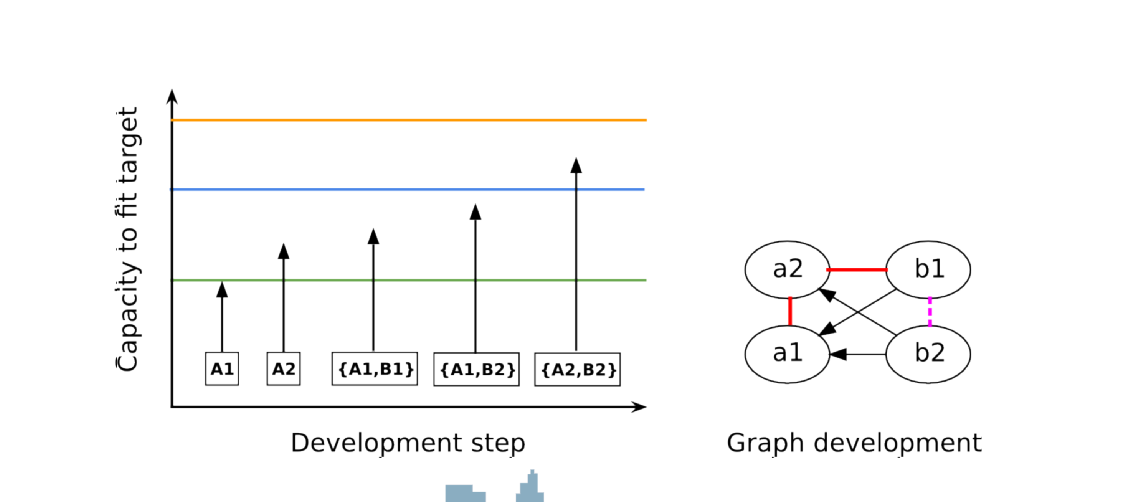
\includegraphics[width=.9\linewidth]{dependance.png}
  \end{sidecaption}
\end{figure}

Comme nous nous situons depuis le début dans une problématique de calibrage par optimisation, dont les résultats n'ont pas vocation d'être transféré de façon directe à une situation réelle, l'apparition d'un nouveau critère venant contraindre la dynamique peut complétement changer la donne dans cette combinatoire des hypothèses plausible. Interpreter de telles situations peut rapidement devenir très complexe : 3 hypothèses peuvent produire une dynamique plus proche des critères que 2 hypothèses, mais 1 hypothèse seule peut apparaitre meilleure que trois hypothèses sur ce même objectif.

Peut-être que la combinaison de ces deux hypothèses est ici la plus intéressante d'un point de vue des questions thématique qu'elle pose, et cela même si la combinaisons des trois hypothèses produit de meilleurs résultat. Peut être qu'à l'introduction d'un nouveau critère, la solution à deux hypothèses produira des meilleurs résultats, et que l'hypothèse 1 verra ses résultats se dégrader ? 

\hl{Schéma ECQTG ?}

Cette interpretation dépend donc du degré de complexification du modèle au moment ou on l'évalue, du nombre de critère retenu pour juger la dynamique, et de la valeur relative que l'on attribue à chacune de ces hypothèses.

Par conséquent aussi cette possibilité de falsification ou \foreignquote{english}{proof of impossibility}, ne marche que si on est en mesure de prouver l'\textbf{inaptitude constante} d'une d'hypothèse ou d'un jeu d'hypothèse dans le rapprochements aux critères. 

Il reste donc à gérer cette possibilité de réengager les hypothèses et les critères à différents moments dans la construction des modèles, et soutenir une activité de construction cumulative qui ne soit pas \enquote{oublieuse} de cette autre espace-temps dans lequel se construise les hypothèses et les différents critères mobilisés. 

